\documentclass[12pt]{article}

\usepackage[margin=1in]{geometry}
\usepackage{amsmath,amssymb,amsthm}
\usepackage{mathtools}
\usepackage{enumitem}
\usepackage{graphicx}
\usepackage{subcaption}
\usepackage{float}
\usepackage{hyperref}
\hypersetup{colorlinks=true,linkcolor=blue,citecolor=blue,urlcolor=blue}
\setlist{itemsep=2pt,topsep=3pt,leftmargin=1.4em}

\theoremstyle{plain}
\newtheorem{theorem}{Theorem}
\newtheorem{lemma}{Lemma}
\newtheorem{proposition}{Proposition}
\theoremstyle{definition}

\newcommand{\norm}[1]{\lVert #1 \rVert}
\newcommand{\dnorm}[1]{\lVert #1 \rVert_{\diamond}}
\newcommand{\tnorm}[1]{\lVert #1 \rVert_{1}}
\newcommand{\ltwo}[1]{\lVert #1 \rVert_{\ell_2}}
\newcommand{\E}{\mathbb{E}}
\newcommand{\Tr}{\operatorname{Tr}}
\newcommand{\ket}[1]{\lvert #1 \rangle}
\newcommand{\ketbra}[1]{\lvert #1 \rangle\!\langle #1 \rvert}
\renewcommand{\Re}{\operatorname{Re}}
\newcommand{\Uchan}{\mathcal{U}}
\newcommand{\Vchan}{\mathcal{V}}
\newcommand{\half}{\tfrac{1}{2}}
\newcommand{\Otil}{\widetilde{O}}

\title{\vspace{-1.3cm}\textbf{Concentration for Random Product Formulas}\\[3pt]
	\large Course Paper --- Theory and Numerical Experiments}
\author{Your Name}
\date{June 19, 2026}

\begin{document}
	\maketitle
	\vspace{-0.5cm}
	
	\begin{abstract}
		\noindent
		This part reconstructs the theory of \emph{Concentration for random product formulas}
		(Chen, Huang, Kueng, Tropp), which analyzes the \textsc{qDRIFT} randomized product formula
		for Hamiltonian simulation. The paper asks whether \textsc{qDRIFT}'s gate count --- famously
		free of explicit dependence on the number $L$ of Hamiltonian terms --- comes from
		\emph{averaging} many random circuits or is already present in \emph{a single} one. The
		answer is the latter: one realization typically approximates the ideal evolution with high
		probability, using $\Otil(n\lambda^2t^2/\epsilon^2)$ gates for a worst-case (diamond-norm)
		guarantee and $\Otil(\lambda^2t^2/\epsilon^2)$ for a fixed input, where $n$ is the qubit
		number and $\lambda=\sum_j\norm{h_j}$. The proof decomposes the error into a deterministic
		bias and a random fluctuation, controlling the latter by a matrix martingale (worst case) or
		a dimension-free vector martingale (fixed input).
	\end{abstract}
	
	
	\section{Setup and the Central Question}
	
	For $H=\sum_{j=1}^{L}h_j$ on $n$ qubits, digital simulation approximates $U=e^{-itH}$ by a
	product $V_N\cdots V_1$ of simple gates, with cost measured by $N$. The first-order
	Lie--Trotter formula $e^{-itH}\approx(e^{-i(t/r)h_L}\cdots e^{-i(t/r)h_1})^{r}$ uses $N=rL$
	gates: each layer must cycle through all $L$ terms, an explicit $L$-dependence that is costly
	when $L$ is large.
	
	\textsc{qDRIFT} (Campbell) avoids this. With $\lambda=\sum_j\norm{h_j}$ and
	$p_j=\norm{h_j}/\lambda$, each step samples one index $j\sim p_j$ and applies
	\begin{equation}
		V_k=\exp\!\Big(-i\tfrac{t}{N}X_k\Big),\quad X_k=\tfrac{\lambda}{\norm{h_j}}h_j\ \text{w.p. }p_j,
		\qquad\text{so}\quad \E[X_k]=\sum_j p_j\tfrac{\lambda}{\norm{h_j}}h_j=H .
		\label{eq:qdrift}
	\end{equation}
	This unbiasedness gives $\E[V_k]\approx e^{-i(t/N)H}=U^{1/N}$, hence by independence
	$\E[V_N\cdots V_1]=(\E V)^N\approx U$. Campbell proved the \emph{averaged channel}
	$\overline\Vchan(\rho)=\E[V_N\cdots V_1\,\rho\,V_1^\dagger\cdots V_N^\dagger]$ is
	$\epsilon$-close to $\Uchan(\rho)=U\rho U^\dagger$ in diamond distance once
	$N=O(\lambda^2t^2/\epsilon)$, with \emph{no} explicit $L$.
	
	That bound concerns the average over circuits, but a user runs the box once and gets a single
	unitary $V_N\cdots V_1$. The paper asks: \emph{does one random circuit already work?} This
	separates \emph{random sampling} from \emph{averaging}. The answer: sampling alone removes
	the $L$-dependence; averaging only improves the accuracy exponent from $1/\epsilon^2$ to
	$1/\epsilon$.
	
	Throughout, $d=2^n$, the generator $(t/N)X_k$ is Hermitian with $\norm{(t/N)X_k}=t\lambda/N$
	(since $\norm{X_k}=\lambda$), and $\Vchan^{(N)}(\rho)=V_N\cdots V_1\rho V_1^\dagger\cdots V_N^\dagger$
	is the single-realization channel. Two error notions arise. For \emph{all} inputs and
	observables (worst case), the relevant quantity for unitary channels is the diamond distance,
	\begin{equation}
		\half\dnorm{\Uchan-\Vchan}
		=\max_{\ket\psi}\half\tnorm{U\ketbra\psi U^\dagger-V\ketbra\psi V^\dagger}
		=\max_{\ket\psi}\max_{\norm{O}\le1}\big|\langle O\rangle_{U\ket\psi}-\langle O\rangle_{V\ket\psi}\big|;
		\label{eq:diamond}
	\end{equation}
	for a single \emph{fixed} input $\rho$, it is the trace distance
	$\half\tnorm{U\rho U^\dagger-V\rho V^\dagger}$.
	
	
	\section{Main Results}
	
	\begin{theorem}[Worst case, diamond norm]\label{thm:diamond}
		Draw $V^{(N)}=V_N\cdots V_1$ from \eqref{eq:qdrift} with
		$N\ge\Omega\big((n+\log(1/\delta))\lambda^2t^2/\epsilon^2\big)$. Then with probability
		$\ge1-\delta$, $\;\max_{\ket\psi}\max_{\norm{O}\le1}|\langle O\rangle_{V^{(N)}\ket\psi}-\langle O\rangle_{U\ket\psi}|<\epsilon.$
		Moreover $\;\E[\half\dnorm{\Uchan-\Vchan^{(N)}}]\lesssim\sqrt{n\lambda^2t^2/N}.$
	\end{theorem}
	
	\begin{theorem}[Fixed input, trace norm]\label{thm:fixed}
		Fix any state $\ket\psi$ and draw $V^{(N)}$ with $N\ge\Omega\big(\lambda^2t^2\log(1/\delta)/\epsilon^2\big)$.
		Then with probability $\ge1-\delta$, $V^{(N)}\ket\psi$ is $\epsilon$-close to $U\ket\psi$ in
		trace distance, and $\;\max_\rho\E[\half\tnorm{\Uchan(\rho)-\Vchan^{(N)}(\rho)}]\lesssim\sqrt{\lambda^2t^2/N}.$
	\end{theorem}
	
	Neither bound contains $L$, so \textsc{qDRIFT}'s $L$-independence already holds for one
	circuit; by the probabilistic method Theorem~\ref{thm:diamond} even proves such $L$-free
	formulas \emph{exist}. The price for a single circuit is accuracy $1/\epsilon^2$ (vs.\
	$1/\epsilon$ for the average), and the worst case carries a factor $n=\log_2 d$. Strikingly,
	fixing the input removes $n$ \emph{without any knowledge of the state} --- only the assumption
	that $\ket\psi$ is chosen independently of the gates; deterministic methods usually need
	spectral structure (e.g.\ a low-energy subspace) for such a gain. Writing $\Otil$ for
	log-suppressed factors, the hierarchy is
	\[
	N_{\mathrm{avg}}=O\big(\tfrac{\lambda^2t^2}{\epsilon}\big)\ \prec\
	N_{\mathrm{fixed}}=\Otil\big(\tfrac{\lambda^2t^2}{\epsilon^2}\big)\ \prec\
	N_{\mathrm{worst}}=\Otil\big(\tfrac{n\lambda^2t^2}{\epsilon^2}\big).
	\]
	The $1/\epsilon$ vs.\ $1/\epsilon^2$ gap is the ``quadratic improvement from mixing,'' an
	instance of Jensen's inequality for the convex distance functional.
	
	
	\section{Proof Strategy}
	
	All regimes share one skeleton: reduce the diamond distance to an operator (or vector) norm,
	split the error as
	\begin{equation}
		\norm{V_N\cdots V_1-U}\le\underbrace{\norm{(\E V)^N-U}}_{\text{deterministic bias}}+\underbrace{\norm{V_N\cdots V_1-(\E V)^N}}_{\text{random fluctuation}},
		\label{eq:decomp}
	\end{equation}
	bound the bias by matrix-exponential estimates plus telescoping, and bound the fluctuation by
	a martingale inequality. Geometrically $V_N\cdots V_1$ is a random walk on $U(d)$: the bias is
	the offset of its mean from $U$, the fluctuation its spread about the mean.
	
	\paragraph{Step 1: diamond $\to$ operator norm.}
	For unitary channels no ancilla is needed, so the diamond distance collapses to a norm.
	
	\begin{lemma}\label{lem:reduction}
		For unitary $\Uchan,\Vchan$ and any pure $\ket\psi$,
		$\half\tnorm{\Uchan(\ketbra\psi)-\Vchan(\ketbra\psi)}\le\ltwo{(U-V)\ket\psi}$, hence
		$\half\dnorm{\Uchan-\Vchan}\le\norm{U-V}$; for the averaged channel,
		$\half\dnorm{\Uchan-\E[\Vchan]}\le2\norm{U-\E V}$.
	\end{lemma}
	\noindent\emph{Proof idea.} Fix $\ket\psi$ and set $\ket u=U\ket\psi$, $\ket v=V\ket\psi$, so
	$|\langle u,v\rangle|\le1$. The Fuchs--van~de~Graaf relation converts the output trace
	distance into a fidelity:
	\[
	\half\tnorm{\ketbra u-\ketbra v}=\sqrt{1-|\langle u,v\rangle|^2}=\sqrt{(1+|\langle u,v\rangle|)(1-|\langle u,v\rangle|)}\le\sqrt{2(1-\Re\langle u,v\rangle)}=\ltwo{\ket u-\ket v}.
	\]
	Maximizing over pure inputs, and using that stabilization (an ancilla) is unnecessary for the
	diamond distance of unitary channels, gives the first two claims. For random $V$ with $E=\E V$,
	expand $\E[V\ketbra\psi V^\dagger]=E\ketbra\psi E^\dagger+\E[(V-E)\ketbra\psi(V-E)^\dagger]$
	(cross terms vanish); bounding the bias term and the positive-semidefinite variance term
	separately, each by $\ltwo{(U-E)\ket\psi}$, yields the factor $2$ (due to Allen--Zhao,
	correcting an earlier claim that omitted it). \hfill$\square$
	
	\paragraph{Step 2: deterministic bias.}
	Using $\norm{e^{iX}-I}\le\norm{X}$ and $\norm{e^{iX}-iX-I}\le\half\norm{X}^2$ for Hermitian
	$X$, with $\norm{(t/N)X_k}=t\lambda/N$ and $\E[(t/N)X_k]=(t/N)H$:
	\begin{equation}
		\norm{V-\E V}\le\tfrac{2t\lambda}{N},\qquad
		\norm{\E V-U^{1/N}}\le\big(\tfrac{t\lambda}{N}\big)^2 .
		\label{eq:singlestep}
	\end{equation}
	The first follows from $\norm{V-\E V}\le\norm{e^{-iX}-I}+\E\norm{I-e^{-iX}}\le2\norm{X}$ (with
	$X=(t/N)X_k$); the second from $\norm{\E V-U^{1/N}}\le\tfrac12\E\norm{X}^2+\tfrac12\norm{\E X}^2\le\E\norm{X}^2$
	via the first-order estimate and Jensen. The single-step bias accumulates by a telescoping
	bound $\norm{(\E V)^N-(U^{1/N})^N}\le N\norm{\E V-U^{1/N}}$ (iterate
	$\norm{A_1A_2-B_1B_2}\le\norm{A_1-B_1}+\norm{A_2-B_2}$ for norm-$\le1$ factors), giving the key
	estimate
	\begin{equation}
		\norm{U-\E[V_N\cdots V_1]}=\norm{(U^{1/N})^N-(\E V)^N}\le\frac{t^2\lambda^2}{N}.
		\label{eq:bias}
	\end{equation}
	This is exactly the averaged-channel bias, $\le\epsilon/2$ once $N\ge2t^2\lambda^2/\epsilon$
	--- already $L$-free with the favorable $1/\epsilon$ rate. Geometrically, the bias is how far
	the random walk's \emph{mean} $(\E V)^N$ sits from the target $U$; the next step controls the
	walk's \emph{spread} about that mean, and the averaged channel pays only the bias --- the root
	of its quadratic accuracy advantage.
	
	\paragraph{Step 3: fluctuation via a matrix martingale.}
	Interpolate between the two ends of \eqref{eq:decomp} by
	\begin{equation}
		B_k=(\E V)^{N-k}V_k\cdots V_1,\qquad B_0=(\E V)^N,\quad B_N=V_N\cdots V_1 .
		\label{eq:mart}
	\end{equation}
	Adjacent iterates differ only at slot $k$, where $\E V$ is replaced by a fresh $V_k$. The
	process is causal and obeys $\E[B_k\mid V_{k-1}\cdots V_1]=(\E V)^{N-k}\E[V_k]V_{k-1}\cdots V_1=B_{k-1}$,
	so it is a martingale. Its increments satisfy
	$\norm{C_k}=\norm{(\E V)^{N-k}(V_k-\E V)V_{k-1}\cdots V_1}\le\norm{V_k-\E V}\le2t\lambda/N=:R$
	and predictable variation $\norm{\sum_k\E_{k-1}C_kC_k^\dagger}\le NR^2=:v$. Matrix Freedman,
	$\operatorname{Pr}[\norm{B_N-B_0}\ge\tau]\le2d\exp(\tfrac{-\tau^2/2}{v+R\tau/3})$, then gives:
	
	\begin{proposition}\label{prop:fluct}
		For $\epsilon\in[0,4t\lambda]$,
		$\;\operatorname{Pr}[\norm{V_N\cdots V_1-\E[V_N\cdots V_1]}\ge\epsilon/2]\le2d\exp(-N\epsilon^2/44t^2\lambda^2).$
		Hence $N\ge(44t^2\lambda^2/\epsilon^2)\log(2d/\delta)$ forces the deviation $\le\epsilon/2$ w.p.\ $\ge1-\delta$.
	\end{proposition}
	
	The error is sub-Gaussian with variance $\sim N(t\lambda/N)^2$, a random walk of $N$ steps of
	size $t\lambda/N$. The prefactor $2d$ is intrinsic to a \emph{matrix}-valued martingale; under
	the log it becomes $\log(2d)=O(n)$ --- the sole source of the system-size factor. Combining
	\eqref{eq:bias} ($\le\epsilon/2$ for $N\ge2t^2\lambda^2/\epsilon$) with
	Proposition~\ref{prop:fluct} ($\log(2d/\delta)=O(n+\log\tfrac1\delta)$) proves
	Theorem~\ref{thm:diamond}; integrating the tail gives the expected bound.
	
	\paragraph{Step 4: fixed input via a vector martingale.}
	For a fixed $\ket\psi$ one compares the output \emph{vectors} $U\ket\psi$ and
	$V_N\cdots V_1\ket\psi$, so \eqref{eq:mart} becomes the vector martingale
	$\ket{\psi_k}=V_k\cdots V_1\ket\psi$. Vector concentration is \emph{dimension-free}; the tool
	is uniform smoothness of the $\ell_2$ norm: if $\E[y\mid x]=0$ then
	$(\E\ltwo{x+y}^q)^{2/q}\le(\E\ltwo{x}^q)^{2/q}+(q-1)(\E\ltwo{y}^q)^{2/q}$ for $q\ge2$. Applied
	recursively across the increments (whose two pieces are conditionally orthogonal) with
	$\E\norm{V_k-\E V_k}^q\le(2t\lambda/N)^q$, it yields
	$(\E\ltwo{(V_N\cdots V_1-\E[\cdots])\ket\psi}^q)^{1/q}\le2\sqrt{(q-1)(t\lambda)^2/N}$. With the
	negligible bias \eqref{eq:bias} and Markov's inequality (optimizing $q$), for $N\ge(t\lambda)^2$,
	\begin{equation}
		\max_\rho\E[\half\tnorm{\Uchan(\rho)-\Vchan^{(N)}(\rho)}]\le4\sqrt{\tfrac{t^2\lambda^2}{N}},\qquad
		\max_\rho\operatorname{Pr}[\half\tnorm{\Uchan(\rho)-\Vchan^{(N)}(\rho)}>\epsilon]\le\exp(-\tfrac{\epsilon^2N}{32e\,t^2\lambda^2}),
		\label{eq:fixed}
	\end{equation}
	which is Theorem~\ref{thm:fixed}. The absence of $d$ here is precisely why the count is
	$n$-free: the dimension-free vector inequality removes the $n$ that
	Theorem~\ref{thm:diamond} pays to cover all $2^n$ inputs at once.
	
	
	\section{Intuition and Generalization}
	
	\paragraph{Why the $n$ appears (and is necessary).}
	For the diagonal commuting Hamiltonian $H=2^{-n}\sum_{p\in\{0,1\}^n}\alpha_p Z_p$
	($\alpha_p\in\{\pm1\}$), $e^{-iH}\ket b=e^{-iS(b)}\ket b$ with phase
	$S(b)=2^{-n}\sum_p c_p(b)$, $c_p(b)\in\{\pm1\}$. Sampling $N$ terms gives the Monte Carlo
	estimate $\widehat S(b)=\tfrac1N\sum_k c_{p_k}(b)$, which by Hoeffding concentrates around
	$S(b)$ with deviation $\sim1/\sqrt N$. For \emph{one} basis state, $N=1/\epsilon^2$ suffices
	(matching Theorem~\ref{thm:fixed}); to control \emph{all} $2^n$ states, a union bound
	multiplies the failure probability by $2^n$, so $N=n/\epsilon^2$ is needed (matching
	Theorem~\ref{thm:diamond}). Thus $n=\log(2^n)$ is the log-count of states controlled at once,
	the same role $\log(2d)$ plays in Proposition~\ref{prop:fluct}. The dependence is tight at
	both extremes: single-site $H=\sum_k Z_k$ gives, via a multinomial central-limit argument, a
	matching lower bound $\E\norm{U-V_N\cdots V_1}\gtrsim\sqrt{(n-1)(t\lambda)^2/N}$, while for the
	all-strings $H=\sum_{p}Z_p$ the diagonal entries become asymptotically independent (a
	Walsh--Hadamard/CLT analysis), making the union bound tight and again forcing $\sqrt n$. Thus
	commuting Hamiltonians saturate the upper bound, so the factor $n$ is not a proof artifact.
	
	\paragraph{Beyond \textsc{qDRIFT}.}
	The proof used only two properties of the random factors $V_k$ approximating $U=U_N\cdots U_1$:
	\emph{causality} (each $V_k$ depends on the past, not the future) and \emph{accurate steps},
	$\norm{V_k-\E_{k-1}V_k}\le a_k$, $\norm{\E_{k-1}V_k-U_k}\le b_k$. The same analysis then gives
	$\dnorm{\Uchan-\Vchan}\le2\sum_k a_k$ (worst case),
	$\E\dnorm{\Uchan-\Vchan}\lesssim\sqrt{n\sum_k a_k^2}+2\sum_k b_k$ (typical),
	$\E\tnorm{\Uchan(\rho)-\Vchan(\rho)}\lesssim\sqrt{\sum_k a_k^2}+2\sum_k b_k$ (fixed input), and
	$\dnorm{\Uchan-\E\Vchan}\le2\sum_k b_k$ (average). The bias is governed by $\sum_k b_k$, the
	fluctuation by $\sqrt{\sum_k a_k^2}$, with $\sqrt n$ only in the worst-case channel norm. This
	covers randomly permuted Suzuki formulas and randomized compiling. A by-product is a sharpened
	mixing lemma, $\dnorm{\Uchan_k-\E\Vchan_k}\le4\norm{U_k-\E V_k}$, removing the $\tfrac12a^2$
	term of the Hastings--Campbell version.
	
	\paragraph{Two conceptual remarks.}
	First, the $1/\epsilon$ vs.\ $1/\epsilon^2$ split mirrors the distinction between
	\emph{weak} and \emph{strong} error for stochastic differential equation solvers: the
	averaged channel tracks $\E[V_N\cdots V_1]$ (a weak, mean quantity, convergence order $1$ in
	$1/N$), whereas a single realization must control $V_N\cdots V_1$ itself (a strong, pathwise
	quantity, order $1/2$). Second, the guarantees are \emph{existential}: Theorem~\ref{thm:diamond}
	shows that a good circuit is sampled with high probability, but certifying that a given drawn
	circuit is accurate is a separate, harder problem --- a gap that motivates a posteriori
	estimators and derandomized (low-discrepancy) constructions. Because the count is quadratic in
	$t$, \textsc{qDRIFT} is most attractive for short-time simulation and for Hamiltonians with
	many terms, where deterministic formulas pay the explicit $L$.

	\section{Numerical Experiments}\label{sec:experiments}

	This section complements the theoretical discussion with direct numerical experiments. The goal is not to fit the constants in the concentration bounds, but to reproduce their qualitative message: a single qDRIFT product formula has a larger error when it must work for all input states, while the fixed-input error is nearly independent of the system size once the Hamiltonian strength $\lambda$ is held fixed.

	\subsection{qDRIFT protocol and error metrics}

	For each Hamiltonian $H=\sum_j h_j$, the experiments use the qDRIFT sampling rule from Eq.~\eqref{eq:qdrift}. At each step, one term is sampled with probability $p_j=\norm{h_j}/\lambda$, where $\lambda=\sum_j\norm{h_j}$, and the short-time unitary
	\[
	V_k=\exp\!\left(-i\frac{t}{N}\frac{h_j}{p_j}\right)
	\]
	is applied. Each plotted point is the average over 50 independent random product formulas. The evolution time is fixed to $t=2$.

	Two errors are measured. For the worst-case setting, the experiment computes the operator norm
	\[
	\epsilon_{\mathrm{all}}=\norm{U-V_N\cdots V_1}_\infty,
	\]
	which controls all input states and all observables through Lemma~\ref{lem:reduction}. For the fixed-input setting, the input state is a tensor product of single-qubit Haar-random states, chosen independently of the qDRIFT gates, and the experiment computes
	\[
	\epsilon_{\mathrm{fixed}}=\ltwo{U\ket\psi-V_N\cdots V_1\ket\psi}.
	\]
	The relative-size plots normalize each curve by its smallest-system value. The dotted line in the all-input relative plot is an empirical linear fit to the measured data, not a theoretical equality; the dotted line in the fixed-input relative plot is the empirical mean, included to show whether the curve is approximately horizontal.

	\subsection{One-dimensional Heisenberg chain}

	The first experiment follows the numerical setting in the paper. The Hamiltonian is the normalized nearest-neighbor Heisenberg chain
	\[
	H=\frac{1}{n-1}\sum_{i=1}^{n-1}\bigl(X_iX_{i+1}+Y_iY_{i+1}+Z_iZ_{i+1}\bigr),
	\]
	where $n=4,5,6,7,8$ is the number of qubits. This normalization gives $\lambda=3$ for all system sizes. The gate counts are $N=20,40,80,120,160,240,320$, and the system-size comparison uses $N=160$.

	\begin{figure}[H]
		\centering
		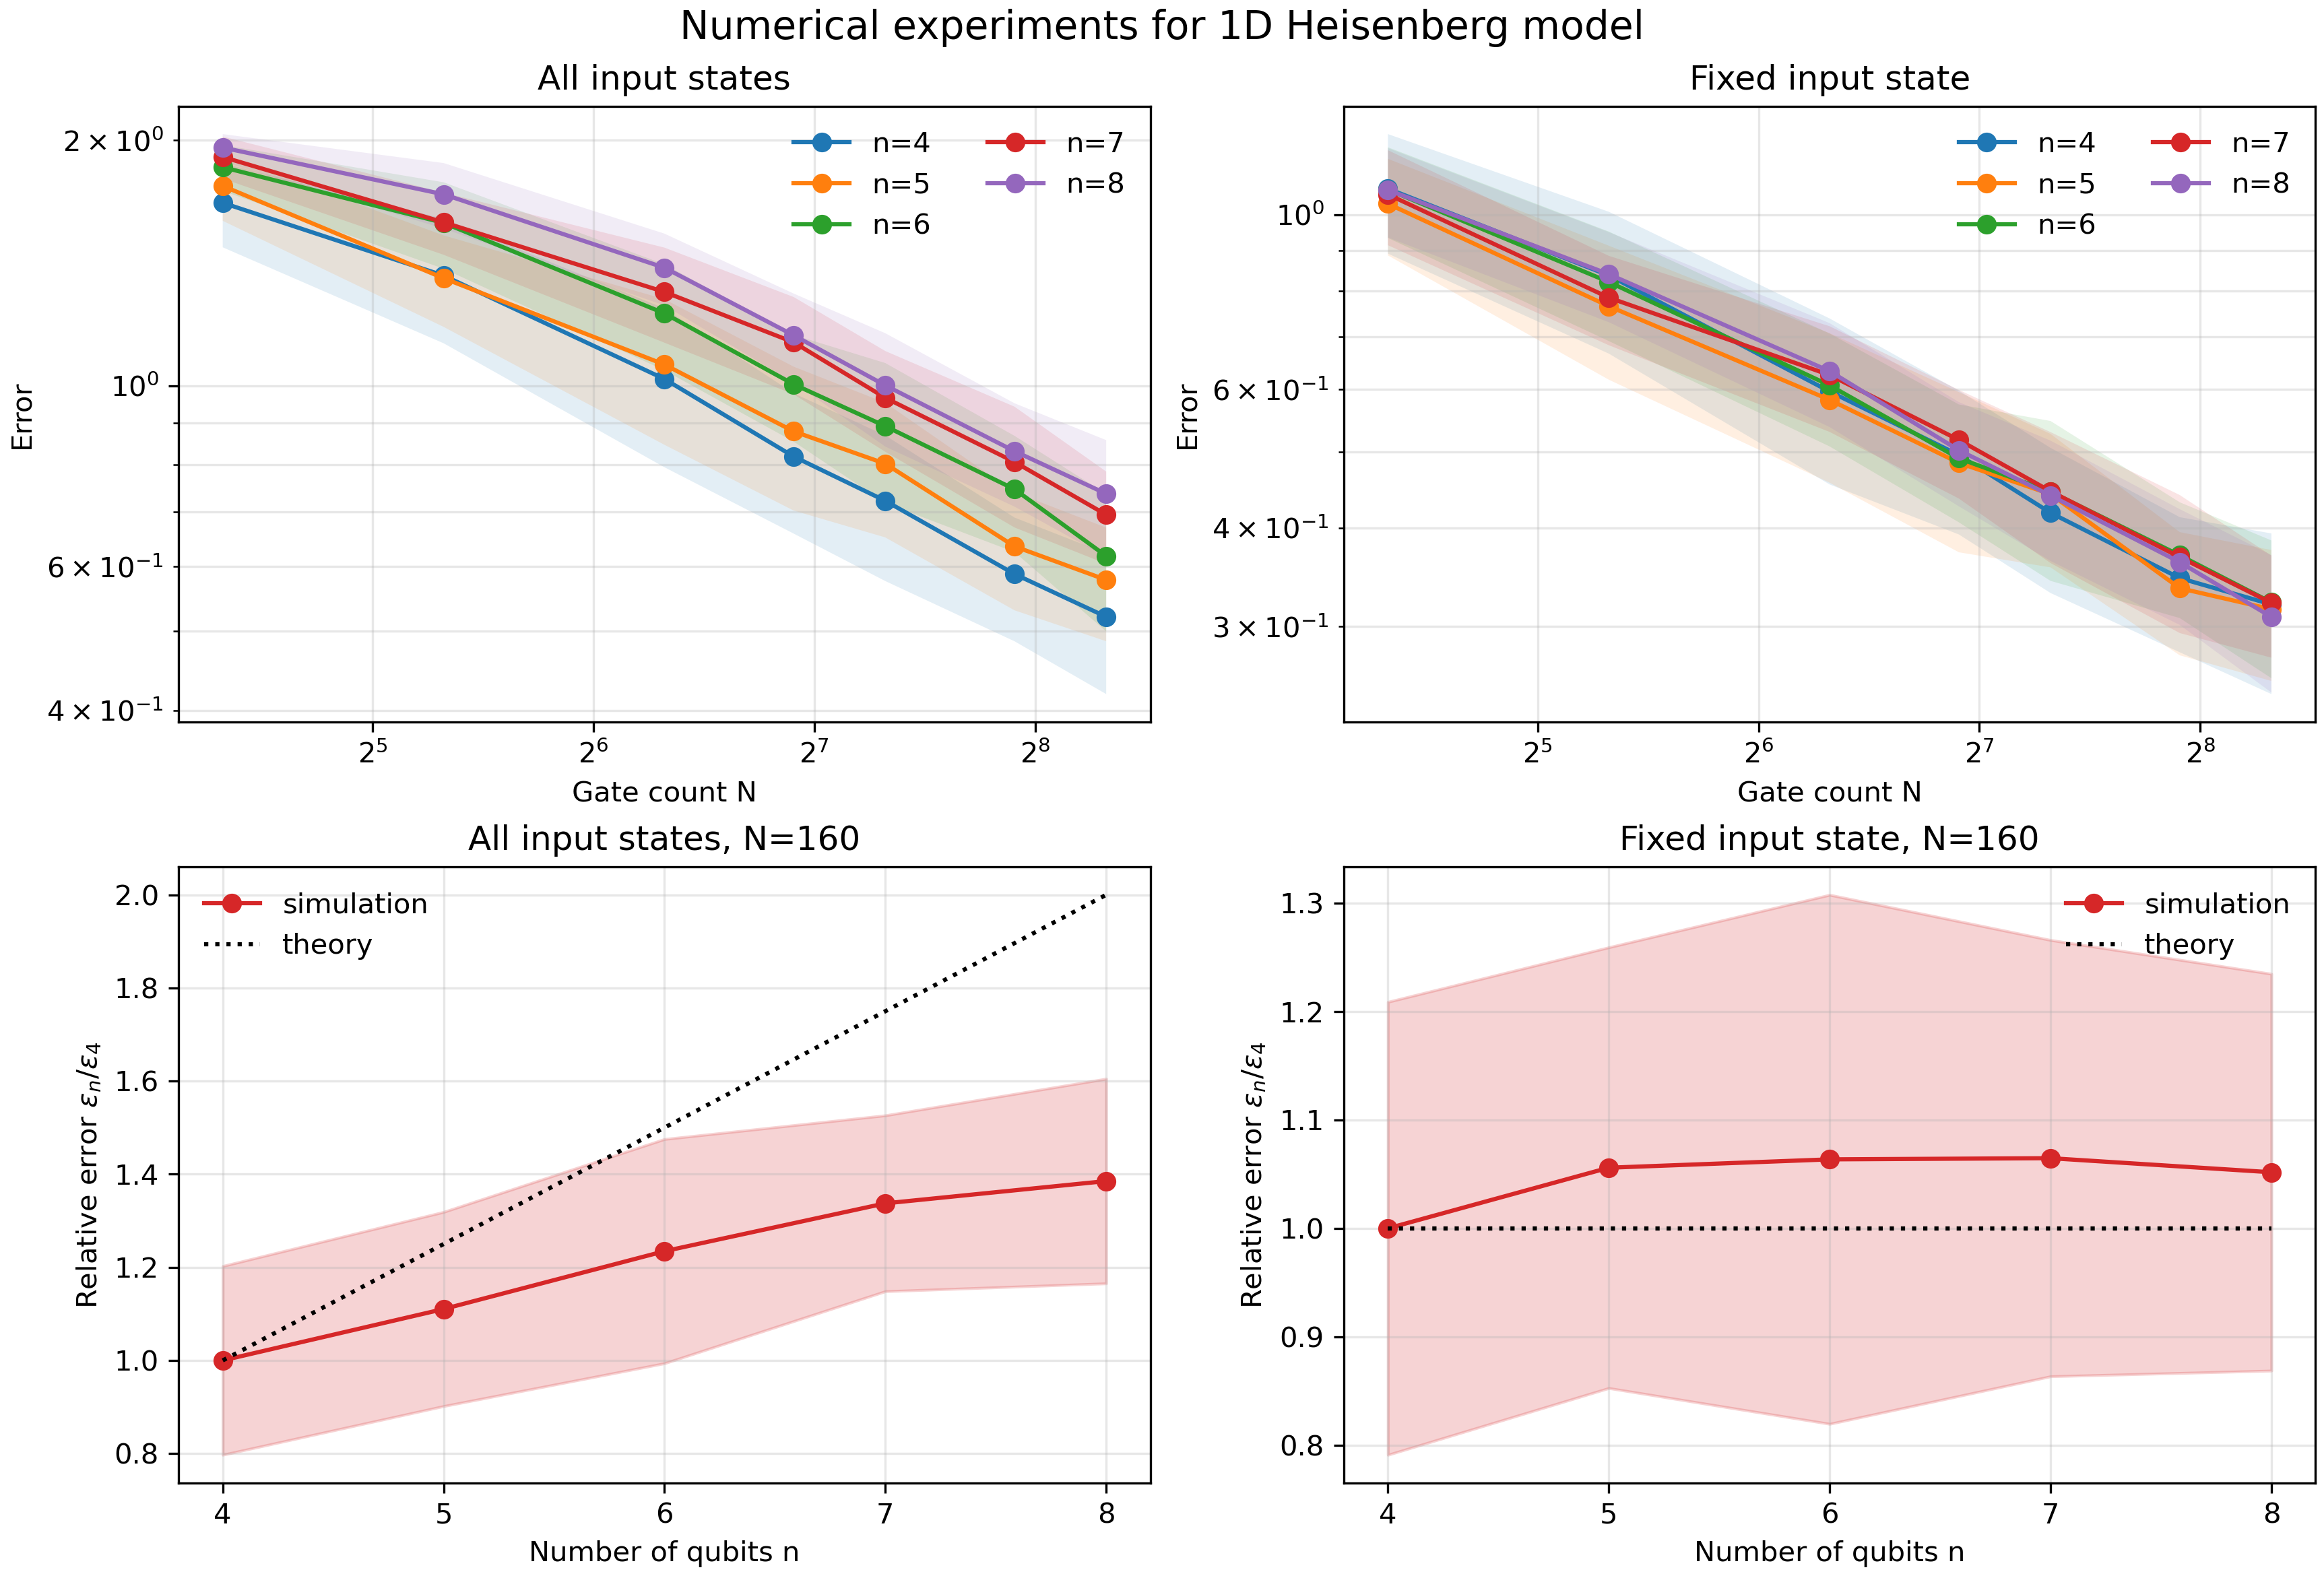
\includegraphics[width=0.95\textwidth]{figures/figure3_reproduction.png}
		\caption{qDRIFT simulation of the normalized one-dimensional Heisenberg chain. The top row compares the decay of the error as the gate count $N$ increases. The bottom row compares the normalized error as the number of qubits increases at fixed $N=160$. The fixed-input error is much flatter than the all-input error, in agreement with the dimension-free fixed-input concentration bound.}
		\label{fig:heisenberg-experiment}
	\end{figure}

	The numerical behavior matches the theory qualitatively. The all-input error increases with the number of qubits at fixed $N$, reflecting the dimension factor in Theorem~\ref{thm:diamond}. By contrast, the fixed-input error remains close to a horizontal trend. This illustrates that the factor $n$ is tied to controlling all possible inputs at once, rather than to the qDRIFT sampling procedure itself.

	\subsection{SYK model}

	The second experiment replaces the Heisenberg Hamiltonian by a Sachdev--Ye--Kitaev (SYK) Hamiltonian. For $n$ Majorana fermions,
	\[
	H=\sum_{1\le i<j<k<l\le n} J_{ijkl}\chi_i\chi_j\chi_k\chi_l,
	\]
	where the couplings are sampled from a centered Gaussian distribution with
	\[
	\overline{J_{ijkl}^2}=\frac{3!J^2}{n^3}.
	\]
	The Majorana operators are represented by the Jordan--Wigner construction
	\[
	\chi_{2r+1}=\frac{1}{\sqrt{2}}Z_1\cdots Z_rX_{r+1},\qquad
	\chi_{2r+2}=\frac{1}{\sqrt{2}}Z_1\cdots Z_rY_{r+1}.
	\]
	Thus $n=8,10,12,14,16$ Majorana modes correspond to $4,5,6,7,8$ qubits. After drawing the Gaussian couplings, the Hamiltonian is rescaled so that $\lambda=3$ for every system size. This extra normalization is important: without it, the qDRIFT strength $\lambda$ grows with the number of SYK terms, and a fixed $N$ comparison would mix system-size effects with a changing Hamiltonian strength.

	\begin{figure}[H]
		\centering
		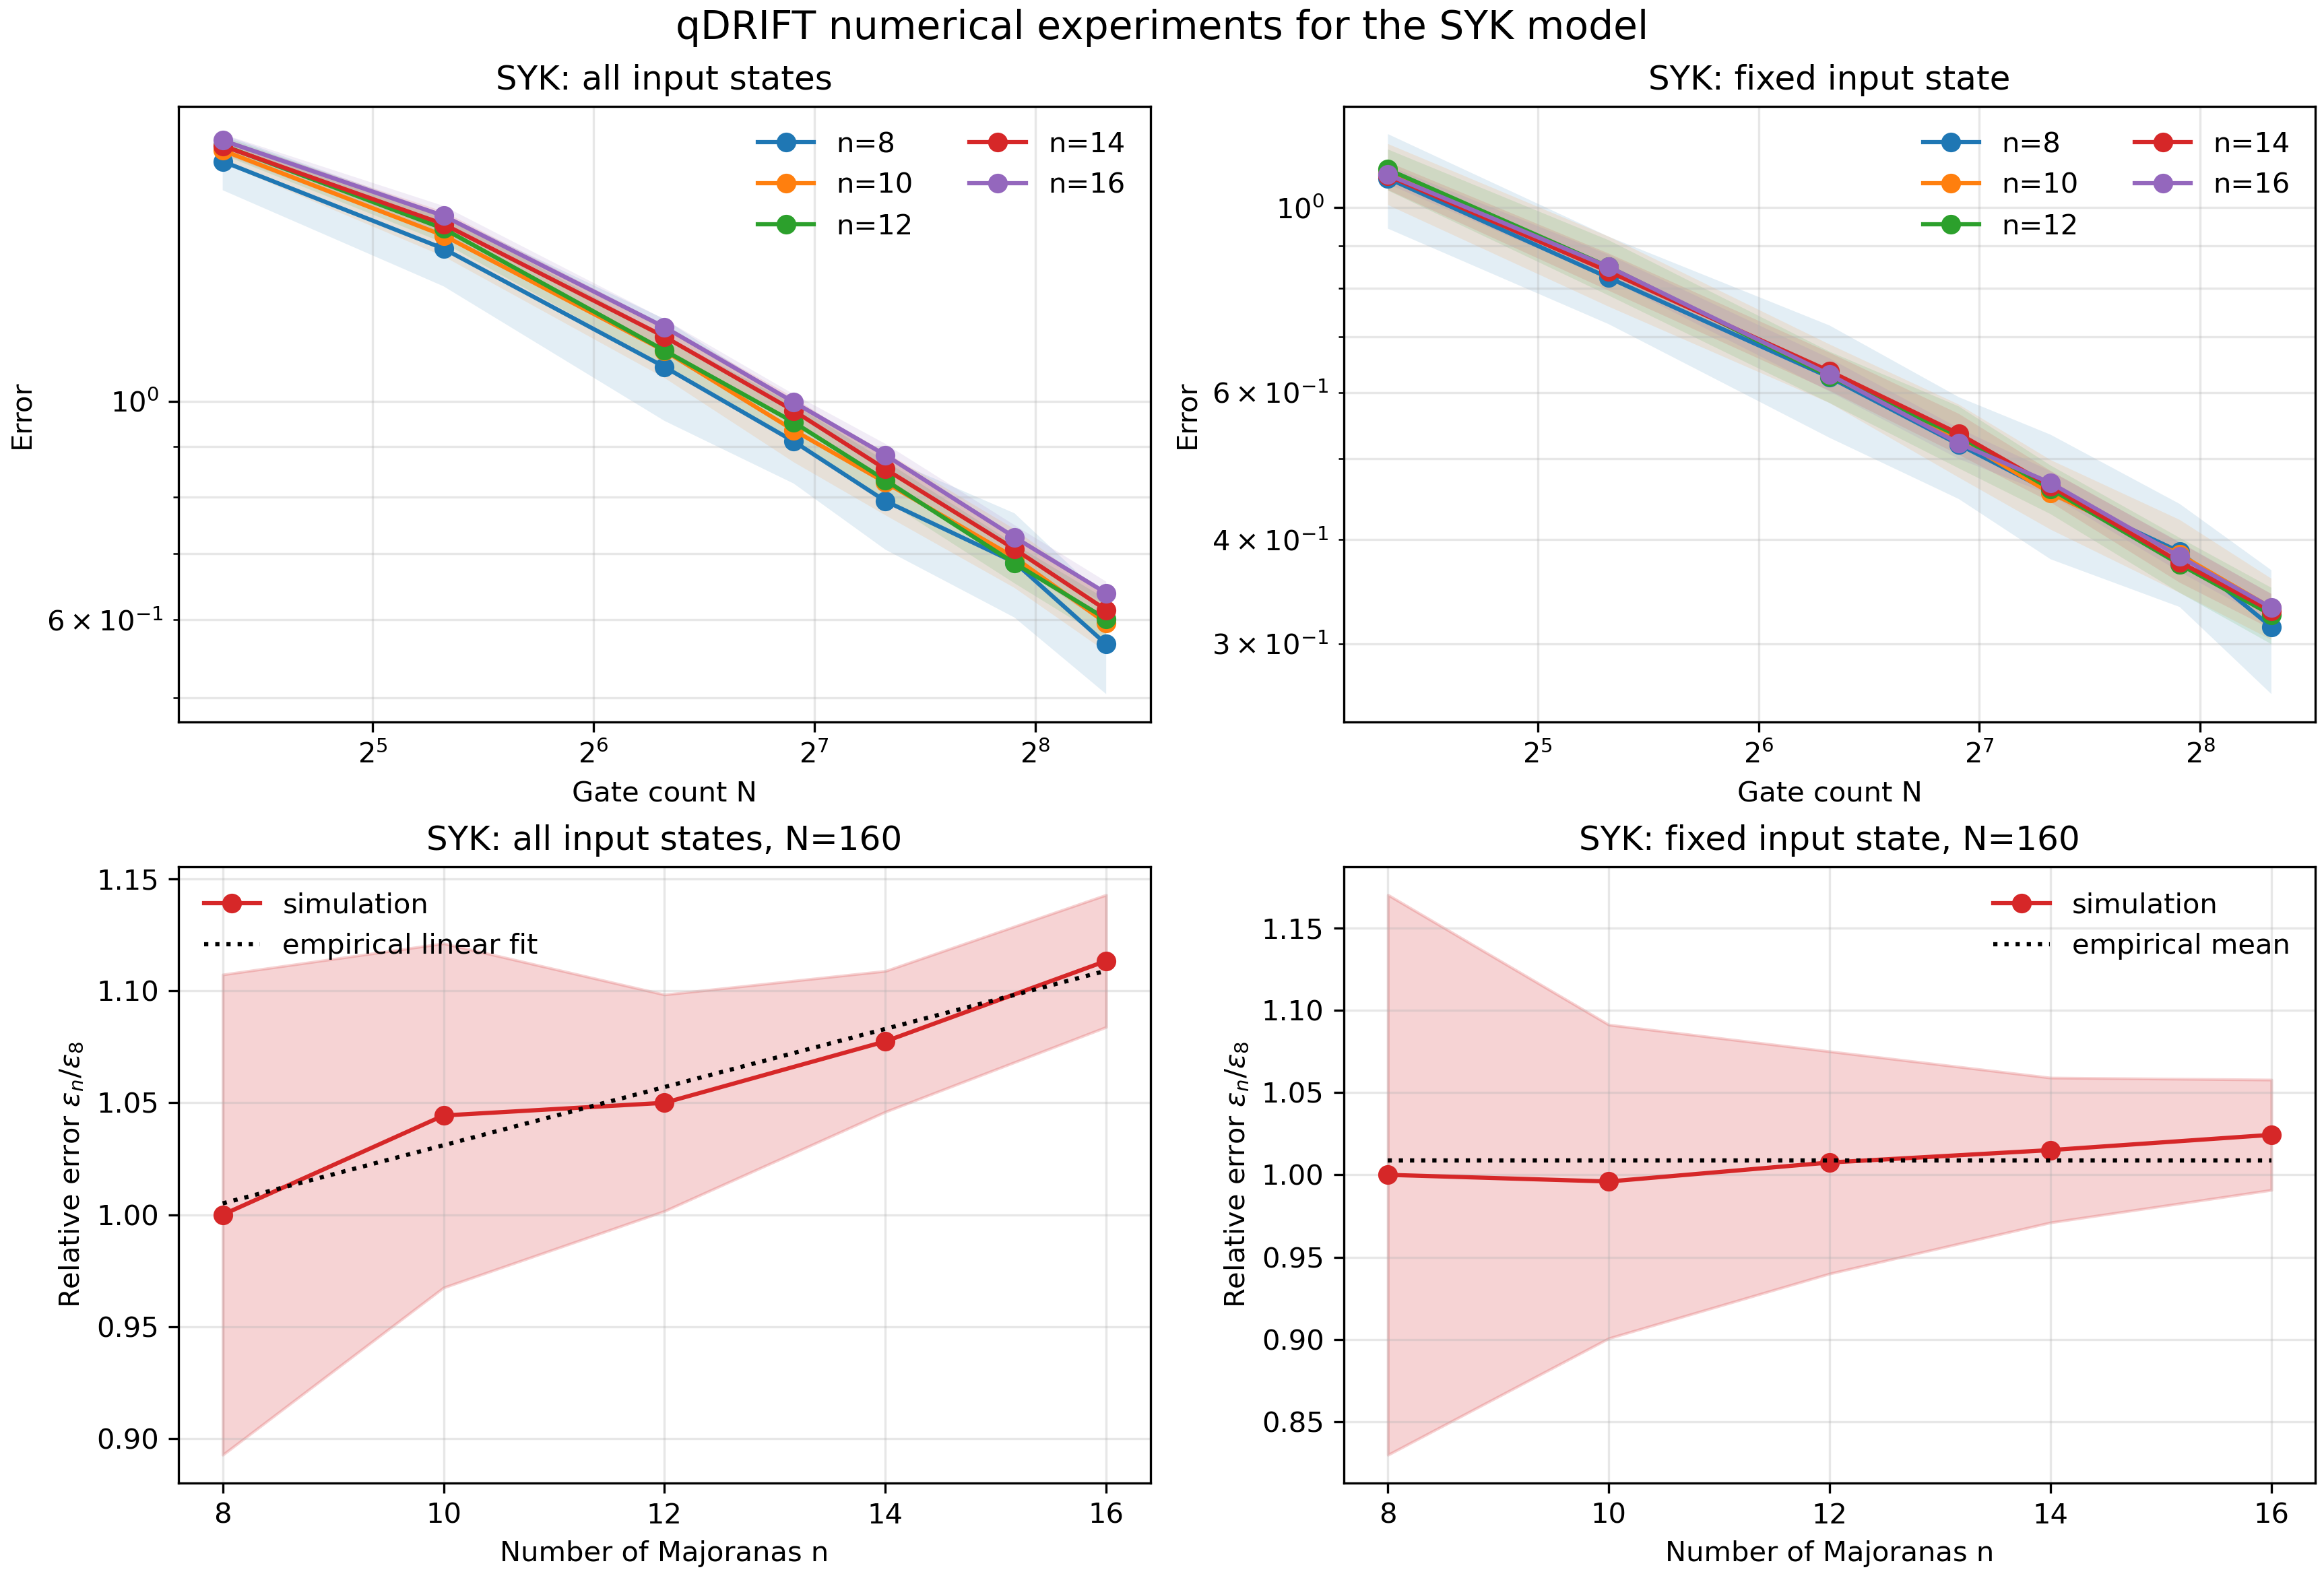
\includegraphics[width=0.95\textwidth]{figures/syk_figure3_style_reproduction.png}
		\caption{qDRIFT simulation of the SYK model after rescaling each instance to $\lambda=3$. The same gate counts and error metrics as in the Heisenberg experiment are used. Once the Hamiltonian strength is fixed, the fixed-input error is again nearly independent of system size, while the all-input error shows a stronger size dependence.}
		\label{fig:syk-experiment}
	\end{figure}

	The SYK experiment confirms that the fixed-input advantage is not special to geometrically local Hamiltonians. Even though the SYK Hamiltonian contains all four-Majorana interaction terms and is highly nonlocal after the Jordan--Wigner mapping, the fixed-input curve remains almost flat once $\lambda$ is normalized. This is consistent with Theorem~\ref{thm:fixed}, whose bound depends on $\lambda$, $t$, and $N$, but not explicitly on the Hilbert-space dimension. The all-input curve, on the other hand, remains more sensitive to system size, as expected from the matrix martingale bound.
	\section{Summary}
	
	Viewing \textsc{qDRIFT} as a random walk on $U(d)$, the error splits into a deterministic bias
	(controlled to $O(t^2\lambda^2/N)$ by matrix-exponential estimates and telescoping) and a
	random fluctuation (controlled to $O(\sqrt{n\,t^2\lambda^2/N})$ by a matrix martingale).
	Restricting to a fixed input replaces the matrix martingale by a dimension-free vector
	martingale, removing $n$ and giving an $n$-fold reduction with no knowledge of the state. The
	$L$-independence of \textsc{qDRIFT} thus stems from random sampling itself; averaging only
	upgrades accuracy from $1/\epsilon^2$ to $1/\epsilon$. Section~\ref{sec:experiments} reproduces the qualitative
	scalings $E_{\mathrm{worst}}\sim\sqrt{n/N}$ and $E_{\mathrm{fixed}}\sim N^{-1/2}$ numerically on Heisenberg and SYK Hamiltonians.
	
	\begin{thebibliography}{9}
		\setlength{\itemsep}{0pt}
		\bibitem{CHKT} C.-F.\ Chen, H.-Y.\ Huang, R.\ Kueng, J.\ A.\ Tropp, \emph{Concentration for random product formulas}, arXiv:2008.11751.
		\bibitem{Campbell} E.\ Campbell, \emph{Random compiler for fast Hamiltonian simulation}, Phys.\ Rev.\ Lett.\ \textbf{123}, 070503 (2019).
		\bibitem{Tropp} J.\ A.\ Tropp, \emph{Freedman's inequality for matrix martingales}, Electron.\ Commun.\ Probab.\ \textbf{16}, 262--270 (2011).
	\end{thebibliography}
	
\end{document}


